%%=============================================================================
%% Resultaten
%%=============================================================================

\chapter{\IfLanguageName{dutch}{Resultaten}{Results}}%
\label{ch:resultaten}

\section{\IfLanguageName{dutch}{Incidenten}{Incidents}}
\label{sec:incidenten-resultaten}

\begin{figure}[h]
    \centering
    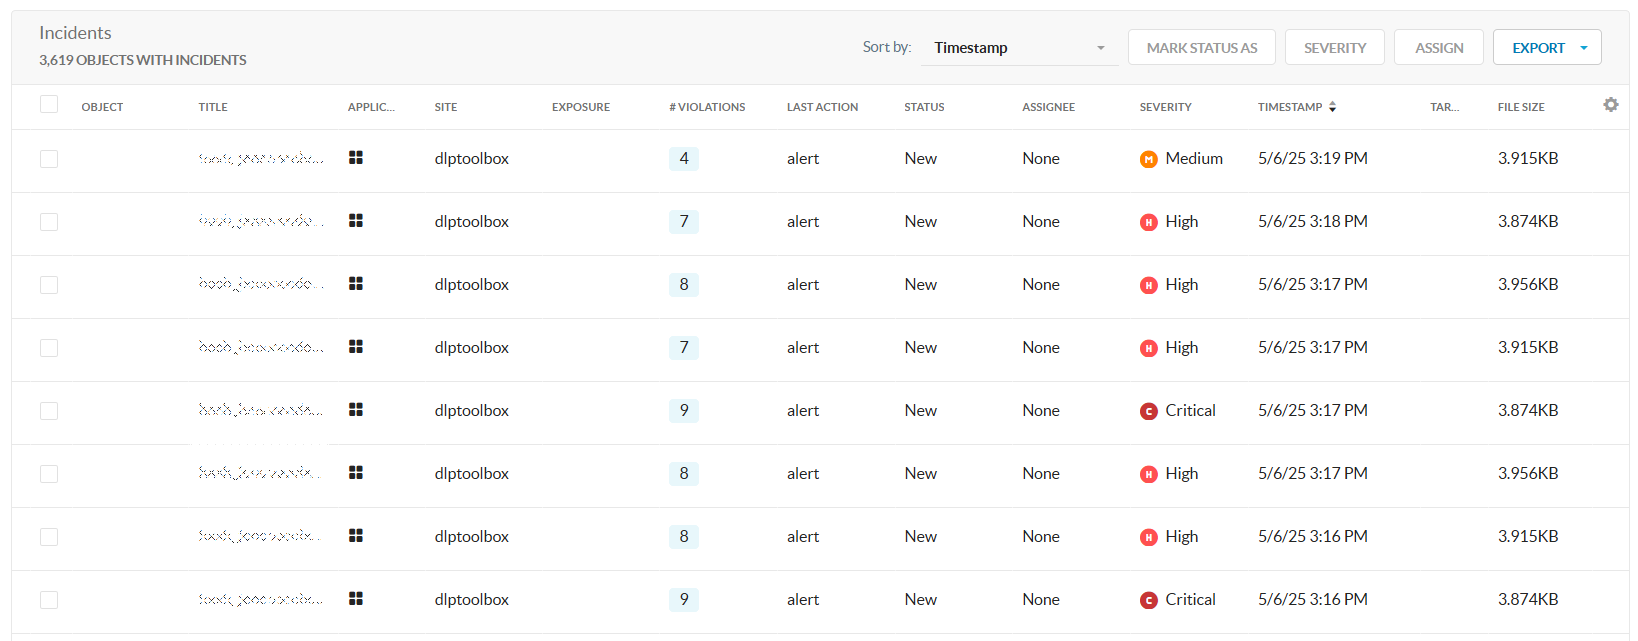
\includegraphics[width=0.8\textwidth]{img/netskope_incidents2.png}
    \caption{Incidenten in Netskope}
    \label{fig:netskope_incidenten}
\end{figure}

\section{\IfLanguageName{dutch}{Vooraf gedefinieerde DLP-regels}{Predefined DLP rules}}
\label{sec:res-vooraf-gedefinieerde-dlp-regels}


\subsection{\IfLanguageName{dutch}{Functionaliteit}{Functionality}}
\label{sec:functionaliteit-resultaten-vooraf}


\subsection{\IfLanguageName{dutch}{Correctheid}{Correctness}}
\label{sec:correctheid-resultaten-vooraf}

Zoals vermeld in Sectie \ref{sec:correctheid} zal de correctheid van de DLP-regels worden geëvalueerd aan de hand van een confusion matrix \ref{tab:confusion_matrix}. 
Tabel \ref{tab:confusion_matrix-vooraf} toont de confusion matrix voor de vooraf gedefinieerde DLP-regels. 
De evaluatieperiode liep van 22 april 2025 tot en met 22 mei 2025. 
In de eerste week werden alle eigen gemaakte regels in een evaluatie modus gezet. 
De eindgebruiker kreeg een melding wanneer er een verwerking van gevoelige data plaatsvond, maar de verwerking werd niet geblokkeerd. 
In dezelfde week en de weken erna werden de regels verder geconfigureerd en getest. 


\begin{table}[h]
    \centering
    \begin{tabular}{|c|c|c|}
        \hline
        \textbf{} & \textbf{Werkelijke Gevoelige Data} & \textbf{Geen Gevoelige Data} \\ \hline
        \textbf{Gedetecteerd als gevoelig} & TP & FP \\ \hline
        \textbf{Niet gedetecteerd als gevoelig} & FN & TN \\ \hline
    \end{tabular}
    \caption{Confusion Matrix voor regex-detectie}
    \label{tab:confusion_matrix-vooraf}
\end{table}


\subsubsection{\iflanguage{dutch}{Hoe eenvoudig is het om de DLP-regels te configureren?}{false}}
\label{}

% Aangezien deze regels vooraf zijn gedefinieerd, kan je dit direct toepassen op de organisatie. 
% Er is bijvoorbeeld geen mogelijkheid om de thresholds te veranderen. 
% Wat lastig kan zijn als je DLP regels wilt toepassen 

1. Niet aanpasbare profielen/regels (Geen mogelijkheid om thresholds te veranderen)
2. Entiteiten zijn niet publiek (moeilijk evalueren als je niet weet wat er mist)

\subsubsection{\iflanguage{dutch}{Is er voldoende documentatie beschikbaar voor de DLP-regels?}{false}}
\label{}

Ja, zoals te merken in dit onderzoek, staat het hier vol mee

\subsubsection{\iflanguage{dutch}{Hoe eenvoudig is het om de DLP-regels te gebruiken?}{false}}
\label{}

Moeilijk met deze

\subsubsection{\iflanguage{dutch}{Is er voldoende ondersteuning beschikbaar voor de DLP-regels?}{false}}
\label{}

Ja, gemakkelijk te clonen om zelf regels aan te maken/ aan te passen

\section{\IfLanguageName{dutch}{Eigen gedefinieerde DLP-regels}{Custom DLP rules}}
\label{sec:res-eigen-gedefinieerde-dlp-regels}


\subsection{\IfLanguageName{dutch}{Functionaliteit}{Functionality}}
\label{sec:functionaliteit-resultaten-eigen}

\subsection{\IfLanguageName{dutch}{Correctheid}{Correctness}}
\label{sec:correctheid-resultaten-eigen}

\textcite{Quaeyhaegens2025}, \textit{Partner Solution Architect} bij \textbf{Netskope}, verklaarde tijdens \textit{Cybersec Europe}: 
``Netskope DLP-incidenten kunnen false positives bevatten, maar genereren nooit false negatives''. 
Deze uitspraak is een persoonlijke notitie. 
DLP-systemen detecteren uitsluitend gegevens die voldoen aan gedefinieerde regels, waardoor relevante matches altijd in beeld komen zolang de configuratie correct blijft.

% Quaeyhaegens2025


\begin{table}[h]
    \centering
    \begin{tabular}{|c|c|c|}
        \hline
        \textbf{} & \textbf{Werkelijke Gevoelige Data} & \textbf{Geen Gevoelige Data} \\ \hline
        \textbf{Gedetecteerd als gevoelig} & TP & FP \\ \hline
        \textbf{Niet gedetecteerd als gevoelig} & FN & TN \\ \hline
    \end{tabular}
    \caption{Confusion Matrix voor regex-detectie}
    \label{tab:confusion_matrix-eigen}
\end{table}

\section{\IfLanguageName{dutch}{Performantie}{Performance}}
\label{sec:performantie-resultaten}


\section{\IfLanguageName{dutch}{Gebruiksvriendelijkheid}{User-friendliness}}
\label{sec:gebruiksvriendelijkheid-resultaten}

% Top Alternatieven voor Netskope DLP
% https://www.nightfall.ai/blog/netskope-dlp-comprehensive-analysis-and-top-alternatives

% The Netskope client uses the same method to inspect and filter traffic that the GlobalProtect App uses to implement domain and application-based split tunneling. The Netskope client can prevent traffic from being sent out the correct interface (VPN virtual interface or physical interface).
% https://knowledgebase.paloaltonetworks.com/KCSArticleDetail?id=kA14u0000001VGGCA2&lang=en_US%E2%80%A9#:~:text=The%20Netskope%20client%20uses%20the,virtual%20interface%20or%20physical%20interface

\section{\IfLanguageName{dutch}{Toekomstig onderzoek}{Future research}}
\label{sec:toekomstig-onderzoek}

% dit heb ik niet onderzocht, ik heb me enkel hierop gericht. stand van zaken, waar zit er een gat?
Tijdens 

